\chapter{Considerações Preliminares} \label{cap:consideracoespreliminares}

Ao longo da execução do trabalho, foi possível perceber que as ferramentas para desenvolvimento multiplataforma 
evoluíram muito desde sua criação, o que as tornaram, hoje, uma opção que deve ser considerada no momento da criação de um novo \textit{app}.

Ambas as abordagens de desenvolvimento móvel possuem suas vantagens e desvantagens, conforme apresentado nos capítulos anteriores desse trabalho. 
No entanto, antigamente as ferramentas \textit{cross} apresentavam um \textit{gap} muito grande quando comparadas às ferramentas e ambientes nativos e com isso, 
dificilmente eram consideradas no momento do desenvolvimento de um aplicativo.

Todas as funcionalidades do aplicativo Mini Farma, que foram planejadas para serem desenvolvidas no ambiente \textit{cross-plataform}, puderam ser desenvolvidas, não havendo quaisquer limitações 
quanto ao uso dos recursos nativos do dispositivo necessários para o projeto selecionado. O \textit{app} multiplataforma se assemelhou muito 
ao nativo em relação a aparência e usabilidade o que confirma a ideia de que as ferramentas multiplataforma estão cada vez mais se aproximando
das nativas apresentando, com o passar do tempo, mais vantagens do que desvantagens, mostrando ainda, que os gargalos antes vistos para essa forma de desenvolvimento, não condizem
mais com a realidade.

Com o término da primeira parte deste trabalho, pôde-se concluir que o desenvolvimento móvel requer uma análise aprofundada de uma série de fatores, 
como mercado, público e tecnologias para decidir qual abordagem escolher.
É importante ressaltar, que a abordagem nativa não é melhor que a \textit{cross-platform} ou vice-versa, sendo apenas distinta e deve-se avaliar qual utilizar caso a 
caso. Para cada situação existem fatores que devem ser avaliados de uma maneira conjunta e alguns desses fatores são listados e explicados a seguir.

\begin{itemize}
    \item \textbf{Tipo e complexidade da aplicação}: cada aplicação possui requisitos diferentes e próprios que originam necessidades e dificuldades inerentes daquele aplicativo. Com isso, deve-se avaliar,
    com base nos requisitos da aplicação, qual abordagem suporta melhor o \textit{app};
    \item \textbf{\textit{Expertise} da equipe nas plataformas e seus ambientes}: cada equipe possui um conjunto único de habilidades e conhecimentos. No momento da escolha de uma abordagem, esses conhecimentos
    devem ser levados em consideração, visto que é a equipe de desenvolvimento que irá conceber o produto final. Se a equipe, possui mais conhecimentos em uma abordagem do que em outra, isso pode ser 
    um indicativo de qual abordagem escolher;
    \item \textbf{Nicho de mercado que se quer atacar}: Cada plataforma móvel (iOS, Android, \textit{Windows Phone}, etc), domina uma parcela do mercado e possui um grupo de usuários com 
    características, opiniões, necessidades e gostos próprios inerentes à plataforma que usam. Com isso, no momento de criar um \textit{app} deve-se pensar para quem é esse aplicativo. Se ele for concebido 
    para suprir uma demanda de um grupo específico, talvez não haja a necessidade de criá-lo para várias plataformas;
    \item \textbf{Prazo de desenvolvimento}: Quanto mais plataformas para atender, maior é o tempo necessário para desenvolver a solução. Se o prazo do projeto for apertado para desenvolvimento de mais de uma solução 
    nativa, há de considerar o desenvolvimento multiplataforma, visto que apenas será codificada uma solução que poderá atender várias plataformas diferentes;
    \item \textbf{Capital disponível para investimento}: Desenvolver para plataformas nativas exige ambiente, infraestrutura e conhecimentos diferentes para cada plataforma. Dessa forma, quanto mais plataformas se 
    quer abarcar, mais custoso o projeto será. Uma solução multiplataforma pode ser mais viável economicamente dependendo da situação;
\end{itemize}

A Figura~\ref{fig:analiseapp} a seguir, resume os fatores que devem ser avaliados no momento da escolha da abordagem de desenvolvimento.
\begin{figure}[H]
  \centering
    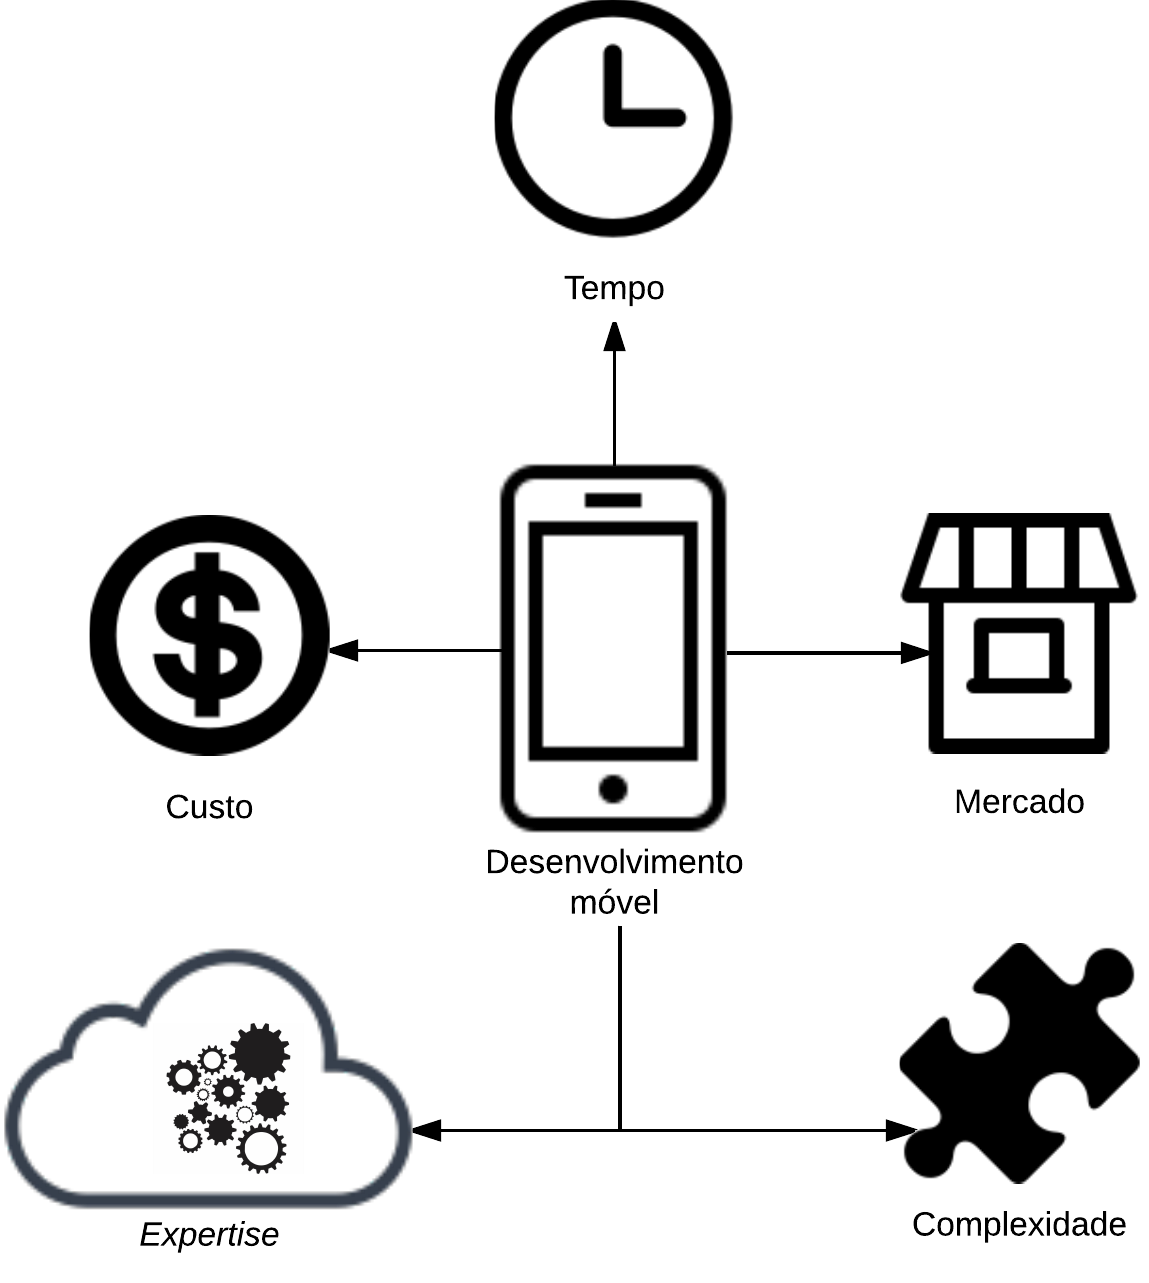
\includegraphics[width=0.5\textwidth]{analiseapp}
    \caption[Fatores a serem avaliados no desenvolvimento móvel]{ Fatores a serem avaliados no desenvolvimento móvel. Fonte: Elaborado pelos autores.}
	\label{fig:analiseapp}
\end{figure}

\section{Planos Futuros} \label{section:planosfuturos}

Na continuação deste trabalho, serão realizadas novas análises de exemplos de uso a fim de obter mais detalhes sobre as vantagens e desvantagens das abordagens de desenvolvimento móvel.
A seguir, é apresentado, na Tabela~\ref{tab:cronograma}, um cronograma preliminar das atividades a serem realizadas.

\begin{table}[h]
\resizebox{\textwidth}{!}{
\begin{tabular}{|l|c|c|c|c|c|c|}
\hline
\multicolumn{1}{|c|}{
\textbf{Atividade}}	                                            & \textbf{Julho} & \textbf{Agosto} & \textbf{Setembro} & \textbf{Outubro} & \textbf{Novembro} & \textbf{Dezembro}   \\ \hline
Recriar um aplicativo nativo Android em Ionic                   & X              & X               & X                  & X               & X                 & X                   \\ \hline
Propor um fluxograma de tomada de decisão                       & X              & X               & X                  & X               & X                 & X                   \\ \hline
Investigar relação com linha de produto de \textit{software}    & X              & X               & X                  & X               & X                 & X                   \\ \hline
Avaliar fluxograma proposto em um projeto Ionic                 & X              & X               & X                  & X               & X                 & X                   \\ \hline
Refinar análise de vantagens e desvantagens e do fluxograma	    & X              & X               & X                  & X               & X                 & X                   \\ \hline
\end{tabular}
}
\caption{Cronograma inicial para o TCC 2}
\label{tab:cronograma}
\end{table}

Será recriado um aplicativo, originalmente feito para a plataforma Android, utilizando o \textit{framework} Ionic a fim de aprimorar o comparativo entre o desenvolvimento nativo e multiplataforma e colher mais insumos
para a proposta de um fluxograma de tomada de decisão de qual abordagem é mais adequada para um dado contexto de desenvolvimento.

Uma vez feito o novo aplicativo, será proposto um fluxograma para auxiliar desenvolvedores a escolher de forma mais assertiva qual abordagem utilizar no contexto de desenvolvimento que estiver imerso.

Realizar pesquisas na área de linha de produto de \textit{software}, para investigar se há alguma relação com o desenvolvimento de aplicativos móveis.

A fim de validar o fluxograma proposto, o mesmo será utilizado em um projeto de evolução de um aplicativo Ionic para avaliar se o modelo de tomada de decisão está correto ou precisa de melhorias.

Ao final serão refinados a análise de vantagens e desvantagens das abordagens de desenvolvimento móvel e o fluxograma criado.